\section*{Introduction}
\addcontentsline{toc}{section}{Introduction}
Au sein de mon cursus d’études d’ingénieurs informatique en apprentissage au CESI de Pau, j’ai commencé mon expérience professionnelle chez Safran Landing Systems (SLS) à Bidos, le 6 octobre 2025, pour une période d’apprentissage de trois ans.

\noindent Cette immersion au sein de l’entreprise me permet de découvrir concrètement le fonctionnement d’une grande organisation industrielle à portée internationale spécialisée dans la conception et l’entretien des systèmes d’atterrissage et de freinage pour l’aéronautique.

\noindent L’objectif de ce rapport d’étonnement est de livrer une analyse de mes premières impressions et observations sur :
\begin{itemize}
  \item Le fonctionnement global de l’entreprise
  \item	L’intégration dans l’environnement de travail
  \item	Les premières missions
  \item	Les points positifs et les axes d’améliorations
\end{itemize}

\noindent En tant que nouvelle apprentie, mon regard extérieur constitue une opportunité pour identifier des éléments à valoriser ou à améliorer, tout en soulignant les enseignements que j’ai déjà tirés de ces premières semaines.

\newpage

\section*{Présentation de l'entreprise}
\addcontentsline{toc}{section}{Présentation de l'entreprise}

\subsection*{Safran Landing Systems}
\phantomsection
\addcontentsline{toc}{subsection}{Safran Landing Systems}

\textbf{Safran Landing Systems} est une filiale du groupe Safran spécialisée dans la conception, le développement, la fabrication et le support des systèmes d’atterrissage et de freinage pour l’aéronautique.

\noindent L’entreprise s’inscrit dans une histoire industrielle de plus d’un siècle, dont les origines remontent à 1909 avec la création de Messier. À la suite de plusieurs évolutions et fusions, notamment avec Dowty, l’entité devient Safran Landing Systems en 2018, marquant son intégration complète au sein du groupe Safran.

\noindent Aujourd’hui, Safran Landing Systems est le \textbf{leader mondial} sur son segment, avec environ \textbf{7 000 collaborateurs} répartis sur plus de \textbf{25 sites industriels dans le monde}. Ses équipements sont présents sur \textbf{un avion sur deux en service}, couvrant l’aviation commerciale, régionale, d’affaires et militaire.

\noindent Le site de \textbf{Bidos}, où s’inscrit mon apprentissage, joue un rôle clé dans cette organisation industrielle, en contribuant à la fabrication et au support de composants critiques pour la sécurité des aéronefs.


\subsection*{Safran Landing Systems - Bidos}
\phantomsection
\addcontentsline{toc}{subsection}{Safran Landing Systems - Bidos}
Le site \textbf{Safran Landing Systems} de \textbf{Bidos}, situé dans les Pyrénées-Atlantiques, constitue l’un des sites industriels historiques du groupe pour les activités liées aux systèmes d’atterrissage. Il regroupe environ un millier de collaborateurs et joue un rôle stratégique dans la fabrication de composants critiques destinés aux trains d’atterrissage d’aéronefs civils et militaires.

\noindent Le site est spécialisé dans l’usinage de pièces de grande dimension, les traitements de surface ainsi que l’assemblage de sous-ensembles à forte valeur ajoutée. Ces activités s’inscrivent dans un environnement industriel fortement contraint par les exigences de sécurité aéronautique, de qualité et de traçabilité, propres au secteur.

\noindent Les productions du site de Bidos sont intégrées à différents programmes majeurs, notamment pour des avionneurs tels qu’Airbus. Du fait de la criticité des pièces produites, chaque étape du processus industriel fait l’objet de contrôles rigoureux et d’un suivi documentaire strict, garantissant la conformité des équipements tout au long de leur cycle de vie. \noindent Intégrer ce site en tant qu’apprentie m’a permis de prendre conscience de la complexité et du niveau d’exigence associés à la production de composants aéronautiques, ainsi que de l’importance du rôle joué par chaque service dans la chaîne de valeur globale.

\section*{Vision d'ensemble}
\addcontentsline{toc}{section}{Vision d'ensemble}

\subsection*{Offres commerciales et prestations}
\phantomsection
\addcontentsline{toc}{subsection}{Offres commerciales et prestations}
Safran Landing Systems propose une offre complète couvrant l’ensemble du cycle de vie des systèmes d’atterrissage et de freinage. Cette offre débute dès la phase de conception, avec le développement de solutions adaptées aux exigences des avionneurs, et se poursuit par la fabrication, l’intégration et les essais des équipements.

\noindent Au-delà de la livraison des systèmes, l’entreprise assure également des prestations de maintenance, de réparation et de révision (MRO), représentant un axe stratégique majeur de son activité. Ces prestations s’inscrivent sur des durées longues, pouvant atteindre plusieurs décennies, et visent à garantir la sécurité, la fiabilité et la disponibilité des aéronefs tout au long de leur exploitation.

\noindent Cette approche globale permet à Safran Landing Systems de se positionner non seulement comme un fournisseur industriel, mais comme un partenaire de long terme pour les compagnies aériennes et les avionneurs.

\subsection*{Clients et partenaires}
\phantomsection
\addcontentsline{toc}{subsection}{Clients et partenaires}
Les principaux clients de Safran Landing Systems sont les grands avionneurs civils et militaires, parmi lesquels figurent notamment Airbus, Boeing, Dassault Aviation, Embraer et Lockheed Martin. Ces clients intègrent les systèmes d’atterrissage dans des programmes aéronautiques majeurs, impliquant des volumes importants et des engagements sur le long terme.

\noindent L’entreprise s’appuie également sur un réseau de partenaires industriels et de sous-traitants, nécessaires à la gestion de chaînes d’approvisionnement complexes et fortement contraintes. Ces partenariats reposent sur des exigences élevées en matière de qualité, de délais et de conformité réglementaire.

\noindent La relation client dans le secteur aéronautique se caractérise ainsi par une forte interdépendance, où la fiabilité industrielle et la capacité à tenir les engagements contractuels sont des facteurs déterminants de pérennité.

\subsection*{Evolutions récentes dans le secteur de l'aviation}
\phantomsection
\addcontentsline{toc}{subsection}{Evolutions récentes dans le secteur de l'aviation}
Le secteur de l’aviation connaît actuellement plusieurs évolutions majeures, influençant directement les activités de Safran Landing Systems. Parmi celles-ci figure la reprise progressive du trafic aérien à la suite des crises récentes, entraînant une augmentation des cadences de production et des besoins accrus en maintenance des flottes existantes.

\noindent Par ailleurs, les enjeux environnementaux occupent une place croissante dans le développement des programmes aéronautiques. Les industriels sont incités à concevoir des équipements plus légers, plus durables et plus facilement réparables, afin de contribuer à la réduction de la consommation de carburant et des émissions associées.

\noindent Enfin, le secteur est marqué par une montée en puissance de la digitalisation des processus industriels, notamment en matière de traçabilité, de maintenance prédictive et de gestion des données, transformant les méthodes de travail et les compétences attendues.

\subsection*{Défis et opportunités}
\phantomsection
\addcontentsline{toc}{subsection}{Défis et opportunités}
Dans ce contexte, Safran Landing Systems fait face à plusieurs défis, notamment la nécessité de maintenir un haut niveau de qualité et de sécurité tout en augmentant les cadences de production. La gestion des compétences, le renouvellement des savoir-faire industriels et l’attractivité des métiers techniques constituent également des enjeux majeurs.

\noindent En parallèle, ces contraintes représentent des opportunités de développement, en particulier à travers l’innovation technologique, l’optimisation des processus industriels et le renforcement des offres de services. La transition vers des pratiques plus durables et l’intégration accrue du numérique ouvrent de nouvelles perspectives pour améliorer la performance globale de l’entreprise.

\noindent En tant qu’apprentie, ces évolutions soulignent l’importance d’une adaptation constante des organisations et confirment l’intérêt de s’inscrire dans un environnement industriel en transformation.

\section*{Organisation de l'équipe}
\addcontentsline{toc}{section}{Organisation de l'équipe}

\subsection*{Composition de l'équipe}
\phantomsection
\addcontentsline{toc}{subsection}{Composition de l'équipe}
Au sein de Safran Landing Systems, j’évolue dans le département \textbf{Qualité}, composé d’environ une \textbf{quarantaine de collaborateurs} aux profils et expertises variés. L’équipe regroupe notamment des responsables qualité, des chargés d’assurance qualité ainsi que des agents de surveillance qualité, intervenant à différents niveaux du processus industriel.

\noindent Cette diversité de fonctions permet de couvrir l’ensemble des enjeux qualité, depuis la définition des exigences et le suivi des procédures jusqu’au contrôle de leur application sur le terrain. Chaque membre de l’équipe apporte des compétences spécifiques, contribuant de manière complémentaire à l’atteinte des objectifs communs.

\newpage

\noindent Mon tuteur, \textbf{Lisandre Marcovici-Soulage}, occupe un rôle central dans mon intégration. Il m’accompagne dans la prise en main des outils, la compréhension des processus internes et la réalisation progressive de mes missions, tout en veillant à mon autonomie croissante.

\subsection*{Répartition des responsabilités}
\phantomsection
\addcontentsline{toc}{subsection}{Répartition des responsabilités}
La répartition des responsabilités au sein du département Qualité est clairement définie, chaque fonction répondant à des missions précises. 

\noindent Les \textbf{responsables qualité} assurent le pilotage global des exigences qualité et la coordination avec les autres services, tandis que les équipes \textbf{d’assurance qualité} veillent à la conformité des processus et au respect des normes en vigueur.

\noindent Les \textbf{agents de surveillance} qualité interviennent quant à eux directement sur le terrain, en lien étroit avec la production, afin de contrôler l’application des procédures et d’identifier d’éventuelles non-conformités. 

\noindent Cette organisation permet une couverture complète du périmètre qualité, depuis les aspects théoriques jusqu’à leur mise en œuvre opérationnelle.

\noindent En tant qu’apprentie, mes responsabilités sont progressivement élargies, sous la supervision de mon tuteur, ce qui me permet de gagner en autonomie tout en évoluant dans un cadre sécurisé

\subsection*{Apprentissage et entraide}
\phantomsection
\addcontentsline{toc}{subsection}{Apprentissage et entraide}
L’environnement de travail au sein du département \textbf{Qualité} est favorable à l’apprentis-sage, notamment grâce à la \textbf{disponibilité des collaborateurs} et à leur volonté de transmettre leurs connaissances. Les échanges sont encouragés, et les membres de l’équipe n’hésitent pas à répondre aux questions ou à expliquer les procédures, les outils et les exigences spécifiques au secteur aéronautique.

\noindent Cet accompagnement s’inscrit toutefois dans une logique d’apprentissage progressif en \textbf{autonomie}. Après une phase d’observation et de prise en main encadrée, il m’est demandé de réaliser certaines tâches de manière \textbf{autonome}, tout en restant soutenue en cas de difficulté. Cette approche me permet de développer mon sens des responsabilités, ma rigueur et ma capacité à prendre des initiatives, tout en respectant un cadre sécurisant.

\noindent L’équilibre entre entraide et autonomie favorise une montée en compétences efficace et réaliste. Il m’a permis de gagner en confiance dans l’exécution de mes missions, tout en comprenant l’importance de la fiabilité et de la précision attendues dans un environnement industriel aussi exigeant que celui de l’aéronautique.

\noindent Cette méthode d'apprentissage contribue à renforcer à la fois la cohésion de l'équipe et la qualité du travail réalisé, en responsabilisant les collaborateurs dès leur intégration.

\section*{Observations générales}
\addcontentsline{toc}{section}{Observations générales}

\subsection*{Intégration dans l'équipe}
\phantomsection
\addcontentsline{toc}{subsection}{Intégration dans l'équipe}
Mon \textbf{arrivée} au sein de l’entreprise a été d’une grande \textbf{facilité} grâce à l’aide mise en place pour les Ressources Humaines de Safran Landing Systems.

oindent Avant mon arrivée j'ai été invitée à utiliser l'outil \textbf{Workelo}. Ce dispositif m'a permis, au fil des jours, de découvrir l'entreprise plus en détail, de préparer mes documents administratifs et d'anticiper mon arrivée en toute sérénité.

\noindent La plateforme propose également des tutoriels très utiles pour se familiariser avec les différents outils de Safran Landing Systems. J'ai ainsi pu découvrir :
\begin{itemize}
  \item \textbf{GTA} : pour la gestion du temps, des pointages et des congés.
  \item \textbf{L'assurance} : pour comprendre les services de protection sociale proposés par l'entreprise.
\end{itemize}

\noindent Ce premier contact digital a grandement facilité les étapes formelles et m'a permis de me sentir accueillie avant même mon premier jour.

oindent Lors de mon arrivée, j'ai pu récupérer mon badge, partir rencontrer l'équipe des ressources humaines ainsi que remplir les derniers documents administratifs.

\noindent On m’a aussi inscrit directement au rendez-vous CSE et visite médicale, ce qui témoigne d’une organisation claire et fluide

oindent A la suite, j'ai pu réaliser une visite de l'usine de l'entreprise avec mon tuteur. Un moment particulièrement marquant afin de comprendre l'identité, le fonctionnement et l'expertise de Safran Landing Systems. Cette introduction a donné un sens concret à mes futures missions.

oindent Cependant, bien que ces étapes aient été formelles et efficaces, l'accès à certains matériels et informations techniques (par exemple, l'accès à des documents internes) a nécessité plus de temps, ainsi qu'un temps d'adaptation non négligeable pour un nouvel arrivant.

\subsection*{Environnement de travail et outils}
\phantomsection
\addcontentsline{toc}{subsection}{Environnement de travail et outils}
L’environnement de travail est similaire à celui des grandes entreprises industrielles. Dès mon arrivée, un ordinateur portable ainsi que les équipements nécessaires m'ont été fournis. Le matériel est déjà configuré pour permettre une prise en main rapide et intuitive par l'utilisateur.

\newpage

\noindent Pour la gestion quotidienne de mon poste de travail, trois outils sont essentiels :
\begin{itemize}
  \item \textbf{Outlook} : pour la gestion des emails et du calendrier professionnel.
  \item \textbf{Teams} : pour la communication interne, les réunions virtuelles et le partage de documents.
  \item \textbf{KeePass} : un logiciel "open source" qui permet de stocker et de gérer tous mes mots de passe dans une base de données sécurisée par un mot de passe unique.
  \item \textbf{Centre de logiciel} : une plateforme interne regroupant tous les logiciels autorisés par l’entreprise, permettant de les installer directement sans solliciter le service informatique.
  \item \textbf{ServiceNow} : une application web pour effectuer toutes mes demandes de matériel, de logiciels ou de droits d’accès, et pour entrer rapidement en contact avec un technicien en cas de problème.
\end{itemize}

\noindent Dans le cadre de mes missions liées à la transformation digitale, j'utilise principalement la suite Microsoft pour analyser et organiser les données :
\begin{itemize}
  \item \textbf{Power BI} : C'est un outil d'analyse de données qui permet de transformer des informations brutes en rapports visuels et interactifs (tableaux de bord) pour faciliter la prise de décision.
  \item \textbf{Microsoft List} : C'est une application de suivi d'informations qui permet de créer des listes intelligentes pour organiser le travail, gérer des inventaires ou suivre des étapes de projets en équipe.
\end{itemize}

\noindent Enfin, pour le développement de projets plus complexes, j'utilise l'éditeur \textbf{Visual Studio Code}. Cet outil me permet de programmer avec différents langages informatiques pour créer des solutions sur mesure adaptées aux besoins du service Qualité.

\subsection*{Remarques}
\phantomsection
\addcontentsline{toc}{subsection}{Remarques}
D’un point de vue global, mon intégration au sein du site de Bidos est très positive. J’ai particulièrement apprécié la bienveillance de l’équipe Qualité, qui a su se rendre disponible pour m'aider à comprendre les enjeux de l'aéronautique.

\noindent Toutefois, j'ai noté quelques points marquants lors de mes premières semaines :
\begin{itemize}
  \item \textbf{Une ambiance de travail saine :} J'ai découvert une équipe soudée où la communication est simple et professionnelle. Malgré le sérieux des missions liées à la sécurité, l'ambiance reste chaleureuse, ce qui est très rassurant pour une personne réservée comme moi.
  \item \textbf{L'entraide au quotidien :} Les collaborateurs n'hésitent pas à partager leurs connaissances et à répondre à mes questions. Cette dynamique favorise un apprentissage serein et permet de gagner rapidement en confiance.
  \item \textbf{La rigueur industrielle :} La visite de l'usine m'a permis de réaliser que chaque donnée informatique que je traite a un impact direct sur la qualité des pièces produites. Cela donne une réelle responsabilité à mes missions.
  \item \textbf{Les délais d'accès :} Comme mentionné précédemment, la sécurité informatique chez Safran impose des délais pour obtenir tous les accès techniques. C’est un point qui demande de la patience lors de l'intégration d'un nouvel arrivant.
\end{itemize}

\section*{Missions}
\addcontentsline{toc}{section}{Missions}

\subsection*{Projet d'apprentissage}
\phantomsection
\addcontentsline{toc}{subsection}{Projet d'apprentissage}
Le but de mon apprentissage au sein de Safran Landing Systems est de participer à la transformation digitale des outils au sein de l'entreprise.

\noindent Ça consiste à intégrer les technologies numériques au cœur des activités d’une entreprise pour améliorer son efficacité. Chez Safran Landing Systems, cela signifie remplacer des processus manuels ou papier par des outils informatiques modernes.

\noindent L'objectif est de rendre les données plus accessibles, de gagner du temps et de réduire le risque d'erreurs. Dans le service Qualité, mon rôle est d'accompagner cette évolution en créant des outils qui permettent de mieux suivre et analyser les informations techniques.

\subsection*{Première mission (27 octobre - 14 novembre 2025)}
\phantomsection
\addcontentsline{toc}{subsection}{Première mission (27 octobre - 14 novembre 2025)}
La première mission qui m'a été confiée consistait à regrouper plusieurs tableaux de bord (\textbf{Dashboards}) Power BI en un seul et unique outil. Auparavant, les informations étaient dispersées sur différents rapports, ce qui rendait le suivi des indicateurs plus long et complexe pour les utilisateurs.

\noindent Ce projet a été piloté et géré principalement par mon tuteur, \textbf{Lisandre Marcovici-Soulage}. De mon côté, je l'ai assisté pour finaliser l'outil, notamment sur la mise en forme et la vérification des données centralisées.

\noindent Cette collaboration m'a permis de :
\begin{itemize}
  \item \textbf{Découvrir concrètement l'utilisation de Power BI} dans un environnement industriel.
  \item \textbf{Comprendre la structure des données} utilisées par le service Qualité.
  \item \textbf{Participer à la simplification du travail de l'équipe} en rendant l'information plus accessible.
\end{itemize}

\newpage

\subsection*{Deuxième mission (22 décembre 2025 - aujourd'hui)}
\phantomsection
\addcontentsline{toc}{subsection}{Deuxième mission (22 décembre 2025 - ...)}
La deuxième mission qui m’a été confiée consiste à développer une application web pour digitaliser des processus qui s'effectuent encore aujourd'hui au format papier. Ce projet s'inscrit directement dans la démarche de transformation digitale du service Qualité

\noindent L'objectif principal est de permettre le remplissage et l'envoi de formulaires numériques pour répondre à plusieurs enjeux :

\begin{itemize}
  \item \textbf{Rapidité :} transmettre instantanément le formulaire aux personnes concernées pour obtenir une signature sans délai de transport physique.
  \item \textbf{Traçabilité :} garantir un suivi précis et sécurisé de chaque document, ce qui est une exigence majeure dans le secteur aéronautique.
  \item \textbf{Productivité :} gagner un temps précieux en automatisant la circulation des informations.
\end{itemize}

\noindent Pour réaliser ce projet plus complexe, j'utilise l'outil Visual Studio Code. Cette mission me permet de mettre en pratique mes compétences en programmation tout en apportant une solution concrète pour améliorer le quotidien opérationnel de l'usine de Bidos.

\section*{Horaires de travail}
\addcontentsline{toc}{section}{Horaires de travail}

Un aspect que j'apprécie vraiment dans ma routine quotidienne est la souplesse des horaires de travail au sein de l'entreprise.

oindent En effet, avoir la possibilité d'arriver le matin entre 7h45 et 8h45, permet à chacun d'organiser son début de journée en fonction de ses propres impératifs personnels ou professionnels. De même pour le départ, qui peut se faire à partir de 16h30 pour ceux ayant accompli leurs 7h12 de travail ou bien se prolonger jusqu'à 19h pour ceux qui préfèrent une journée plus étirée dans le temps.

oindent La pause déjeuner, représente également un moment de liberté apprécié par beaucoup, sa durée est de 30min minimum et peut varier jusqu'à 1h45 maximum, pour s'offrir une pause plus ou moins longue en fonction de la charge de travail ou des besoins du jour.

\noindent Cette souplesse favorise une gestion optimale du temps et contribue à trouver un équilibre plaisant entre vie professionnelle et personnelle.

\newpage

\section*{Points positifs}
\addcontentsline{toc}{section}{Points positifs}
\begin{itemize}
  \item \textbf{Environnement de travail}, le site de Bidos offre un cadre industriel impressionnant et stimulant
  \item \textbf{Encadrement et accompagnement}, mon tuteur, Lisandre Marcovici-Soulage, assure un suivi régulier qui facilite ma compréhension des processus complexes de l'aéronautique. La bienveillance globale de l'équipe Qualité m'aide à surmonter ma timidité et à poser mes questions librement.
  \item \textbf{Missions stimulantes et formatrices}, les projets de transformation digitale sont concrets et motivants. Ils me permettent de voir l'impact direct de mon travail sur la productivité du service.
  \item \textbf{Progression structurée et responsabilités}, l'entreprise propose un équilibre parfait entre l'observation assistée et l'autonomie progressive. Cela me permet de prendre des responsabilités tout en me sentant soutenue en cas de difficulté.
  \item \textbf{Valorisation des compétences analytiques}, face aux défis rencontrés, j’ai appris à mettre en œuvre une logique et des méthodologies rigoureuses pour organiser des données brutes. Cette démarche me permet de transformer ces informations en outils utiles à l'équipe, tout en développant mon esprit d'analyse.
\end{itemize}

\section*{Axes D'amélioration}
\addcontentsline{toc}{section}{Axes D'amélioration}
\textbf{Documentation simplifiée pour les nouveaux arrivant }: En complément de l’outil \textbf{Workelo} proposé par le service Ressources Humaines, qui présente clairement les applications administratives, il serait bénéfique de mettre en place un guide similaire pour les ressources techniques (plateformes académiques, bibliothèques, etc.). S'inspirer de cette méthode permettrait aux nouveaux arrivants de mieux s'orienter parmi les outils informatiques et de gagner en autonomie plus rapidement sur les processus internes.
	
\textbf{Centralisation de l'information }: À ce jour, le site de Bidos utilise un grand nombre de sites \textbf{SharePoint} différents. Je trouve que cette dispersion rend la recherche d'informations complexe et peu claire pour les utilisateurs.
\noindent Il serait, selon moi, plus efficace de créer un \textbf{SharePoint unique pour Safran Landing Systems Bidos}. Ce portail central regrouperait l'ensemble des liens et ressources sur une seule et même plateforme principale. Une telle centralisation éviterait de se perdre entre les différents sites existants et faciliterait grandement l'accès aux documents pour tous les collaborateurs.

\section*{Analyse SWOT}
\addcontentsline{toc}{section}{Analyse SWOT}

\begin{center}
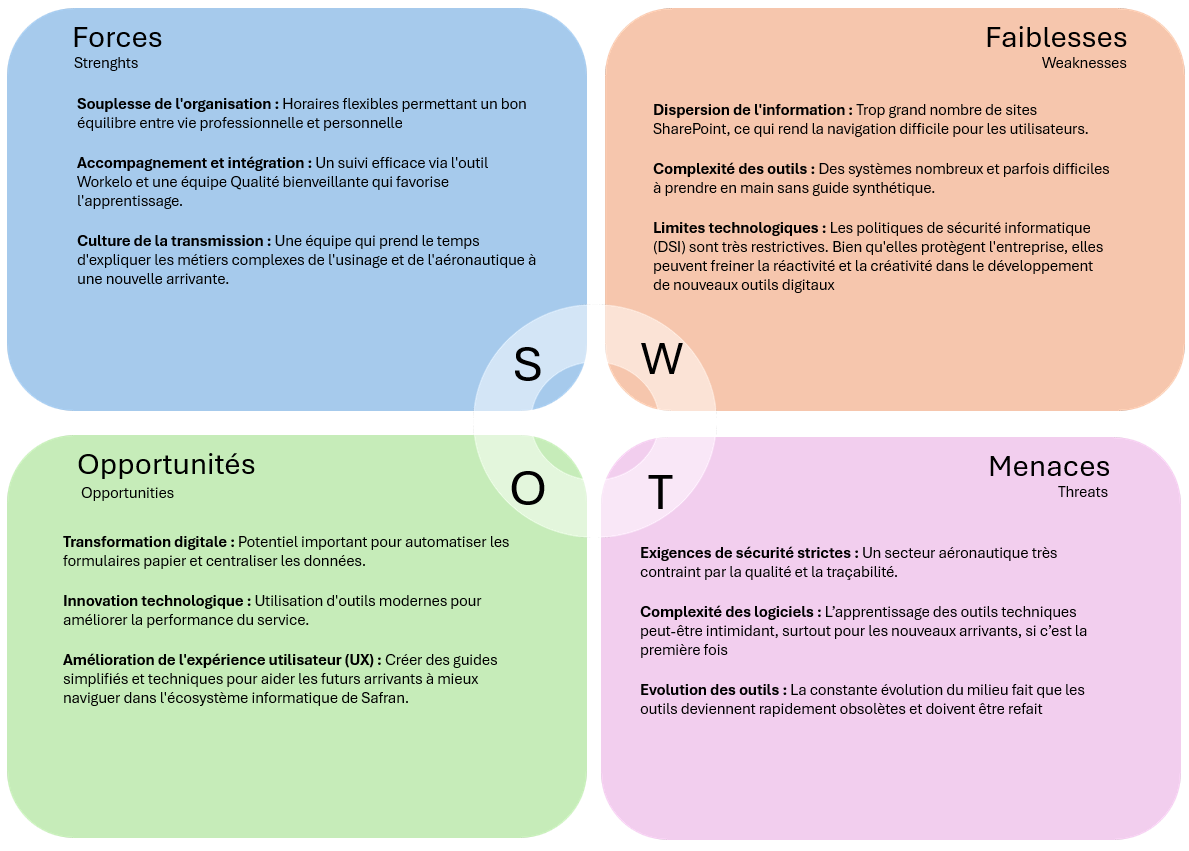
\includegraphics[width=0.9\textwidth]{contents/img/swot.png}
\end{center}

\section*{Conclusion}
\addcontentsline{toc}{section}{Conclusion}
Ces premières semaines chez Safran Landing Systems à Bidos ont été extrêmement enrichissantes. Malgré l’appréhension légitime que l’on peut ressentir lors d’une première immersion dans une grande entreprise industrielle, j’ai été accueillie avec bienveillance par l’équipe Qualité.

\noindent Ce rapport m’a permis de mettre en avant les points forts de mon intégration, notamment l’accompagnement de mon tuteur et la modernité des outils de travail. Les premières missions qui m’ont été confiées sur Power BI et le développement d’une application web confirment mon envie de participer activement à la transformation digitale de l'entreprise.

\noindent Certes, des défis restent à relever, comme la navigation dans l'écosystème informatique ou l’adaptation aux contraintes de sécurité. Cependant, ces obstacles sont autant d'opportunités pour moi de développer ma logique et mon esprit d'analyse.

\noindent Je suis fière de commencer mon cursus d’ingénieur au sein d'un leader mondial comme Safran. Je repars de cette période d'étonnement avec une vision claire de mes responsabilités et une grande motivation pour la suite de mes trois années d'apprentissage.

\newpage
\section*{Sitographie}
\addcontentsline{toc}{section}{Sitographie}
\begin{itemize}
  \item \textbf{Safran Group} : \url{https://www.safran-group.com/fr}
  \item \textbf{Safran Landing Systems} : \url{https://www.safran-landing-systems.com/fr}
  \item \textbf{Analyse SWOT} : \url{https://bpifrance-creation.fr/encyclopedie/letude-marche/determiner-sa-strategie/swot-loutil-danalyse-strategique-developper}
  \item \textbf{Microsoft Power BI} : \url{https://powerbi.microsoft.com/fr-fr/}
  \item \textbf{Visual Studio Code} : \url{https://code.visualstudio.com/}
  \item \textbf{Microsoft SharePoint} : \url{https://www.microsoft.com/fr-fr/microsoft-365/sharepoint}
  \item \textbf{ServiceNow} : \url{https://www.servicenow.com/}
  \item \textbf{KeePass Password Safe} : \url{https://keepass.info/}
\end{itemize}

\newpage
\section*{Glossaire}
\addcontentsline{toc}{section}{Glossaire}
\begin{itemize}
  \item \textbf{CESI} : École d’ingénieurs où je suis ma formation en informatique.
  \item \textbf{CSE (Comité Social et Économique)} : Instance qui représente le personnel de l’entreprise et gère les activités sociales et culturelles.
  \item \textbf{Dashboard} : Tableau de bord permettant de visualiser des données de manière graphique.
  \item \textbf{DSI (Direction des Systèmes d'Information)} : Service responsable de l’ensemble du matériel et des logiciels informatiques de l’entreprise.
  \item \textbf{GTA (Gestion du Temps et des Activités)} : Outil permettant de gérer les temps de travail, les pointages et les absences.
  \item \textbf{KeePass} : Logiciel sécurisé de gestion de mots de passe.
  \item \textbf{MRO (Maintenance, Repair and Overhaul)} : Activités de maintenance, de réparation et de révision des équipements aéronautiques.
  \item \textbf{Open Source} : Se dit d'un logiciel dont le code est accessible et modifiable par tous.
  \item \textbf{Power BI} : Outil de Microsoft utilisé pour analyser des données et créer des rapports visuels.
  \item \textbf{ServiceNow} : Plateforme utilisée pour gérer les demandes d’assistance et les besoins techniques auprès de la DSI.
  \item \textbf{SharePoint} : Outil collaboratif de Microsoft permettant de stocker, partager et organiser des documents au sein d'une équipe.
  \item \textbf{SLS} : Safran Landing Systems.
  \item \textbf{Visual Studio Code (VS Code)} : Éditeur de code utilisé par les développeurs pour écrire et tester des programmes informatiques.
  \item \textbf{Workelo} : Plateforme digitale utilisée pour faciliter l’intégration des nouveaux arrivants (pré-boarding).
\end{itemize}